\documentclass[12pt]{article}
\usepackage[T1]{fontenc}
\usepackage[polish]{babel}
\usepackage[utf8]{inputenc}
\usepackage{graphicx}
\usepackage{amsfonts}
\usepackage{amsmath}
\usepackage{float}
\usepackage{hyperref}

\newcommand{\BibTeX}{{\sc Bib}\TeX} 
\setlength{\textheight}{21cm}

\title{{\bf Zadanie nr 2 -- Próbkowanie i kwantyzacja}\linebreak
Cyfrowe Przetwarzanie Sygnałów}

\author{Łukasz Murza, 251592 \and Aleksander Kaźmierczak, 251544}
\date{20.04.2026}

\begin{document}

\maketitle
\thispagestyle{empty}
\newpage
\setcounter{page}{1}

\section{Cel zadania}
Celem zadania jest empiryczne zbadanie zjawisk i mechanizmów zachodzących podczas zamiany sygnałów ciągłych na postać dyskretną (konwersja A/C) oraz ich ponownej rekonstrukcji do postaci analogowej (konwersja C/A).

\section{Wstęp teoretyczny}
Przejście z sygnałów ciągłych do dziedziny cyfrowej wymaga przeprowadzenia konwersji analogowo-cyfrowej (A/C), na którą składa się próbkowanie w czasie oraz kwantyzacja amplitudy \cite{1}. Próbkowanie równomierne dyskretyzuje sygnał z zadaną częstotliwością, natomiast kwantyzacja (realizowana poprzez obcięcie lub zaokrąglenie) przypisuje próbkom wartości z ograniczonej puli poziomów, co wprowadza nieodwracalny szum kwantyzacji.

Procesem odwrotnym jest konwersja cyfrowo-analogowa (C/A), pozwalająca na rekonstrukcję pierwotnego przebiegu. W tym celu wykorzystuje się metody takie jak ekstrapolacja zerowego rzędu (ZOH) czy rekonstrukcja w oparciu o funkcję Sinc \cite{1}. Aby obiektywnie ocenić jakość odwzorowania oraz wpływ wybranych parametrów na zniekształcenia, stosuje się miary błędów. Należą do nich błąd średniokwadratowy (MSE), stosunek sygnału do szumu (SNR i PSNR), maksymalna różnica (MD) oraz wyznaczana na ich podstawie efektywna liczba bitów (ENOB) \cite{1}.

\section{Instrukcja obsługi aplikacji}
\begin{enumerate}
    \item \textbf{Generacja:} Należy wybrać typ sygnału z listy rozwijanej (np. Sygnał Sinusoidalny), uzupełnić parametry w formularzu i kliknąć przycisk \textit{Generuj}.
    \item \textbf{Rekonstrukcja:} W panelu konwersji, ustalić nową częstotliwość próbkowania oraz liczbę bitów kwantyzacji, wybrać pożądaną metodę z listy (np. Ekstrapolacja zerowego rzędu lub Rekonstrukcja Sinc) i nacisnąć przycisk \textit{Wykonaj konwersję}. Wyniki zostaną wyświetlone na wykresach wraz z obliczonymi miarami błędów.
\end{enumerate}

\section{Eksperymenty i wyniki}

\subsection{Wpływ nowej częstotliwości próbkowania na rekonstrukcję sygnału}
Cel: zbadanie wpływu doboru częstotliwości próbkowania w połączeniu z metodą ekstrapolacji zerowego rzędu (ZOH).\cite{1}.


\begin{table}[H]
    \centering
    \vspace{0.2cm}
    \begin{tabular}{|l|c|}
        \hline
        \textbf{Parametr} & \textbf{Wartość} \\ \hline
        Amplituda ($A$) & 1.0 \\ \hline
        Czas początkowy ($t_1$) [s] & 0.0 \\ \hline
        Czas trwania ($d$) [s] & 1.0 \\ \hline
        Częstotliwość próbkowania ($f$) [kHz] & 10 \\ \hline
        Częstotliwość sygnału [Hz] & 10.0 \\ \hline
        Przesunięcie fazowe [rad] & 0.0 \\ \hline
    \end{tabular}
    \caption{Parametry oryginalnego sygnału}
    \label{tab:prametry_oryginalnego_sygnalu}
\end{table}

\begin{figure}[H]
    \centering
    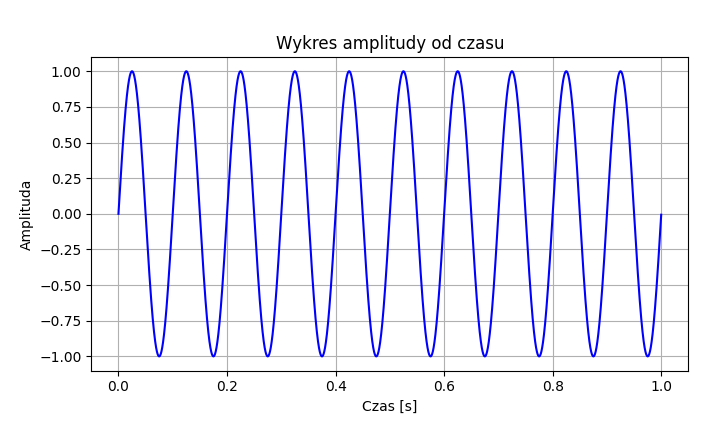
\includegraphics[width=0.85\linewidth]{exp1/original.png}
    \caption{Wykres oryginalnego sygnału.}
    \label{fig:wykres_oryginalnego_sygnalu}
\end{figure}



W czasie trwania eksperymentu zostały zbadane częstotliwości próbkowania podczas rekonstrukcji. Zostały one przedstawione wraz z wynikami miar błędów w poniższych tabelach.


% new_f = 10 Hz
% MSE: 0.5000
% SNR: 0.0000 dB
% PSNR: 3.0103 dB
% MD: 1.0000
% ENOB: -0.2924 bitów

\begin{table}[H]
    \centering
    \vspace{0.2cm}
    \begin{tabular}{|l|c|}
        \hline
        \textbf{Parametr} & \textbf{Wartość} \\ \hline
        \multicolumn{2}{|c|}{\textit{Parametry wejściowe}} \\ \hline
        Częstotliwość próbkowania ($f$) [Hz] & 10.0 \\ \hline
        Liczba bitów kwantyzacji (b) & 8 \\ \hline

        \multicolumn{2}{|c|}{\textit{Miary błędów}} \\ \hline
        MSE & 0.5 \\ \hline
        SNR ($dB$) & 0.0 \\ \hline
        PSNR ($dB$) & 3.0103 \\ \hline
        MD & 1.0 \\ \hline
        ENOB (b) & -0.2924 \\ \hline
    \end{tabular}
    \caption{Parametry i miary błędów po konwersji}
    \label{tab:wyniki_rekonstrukcji_10Hz}
\end{table}

\begin{figure}[H]
    \centering
    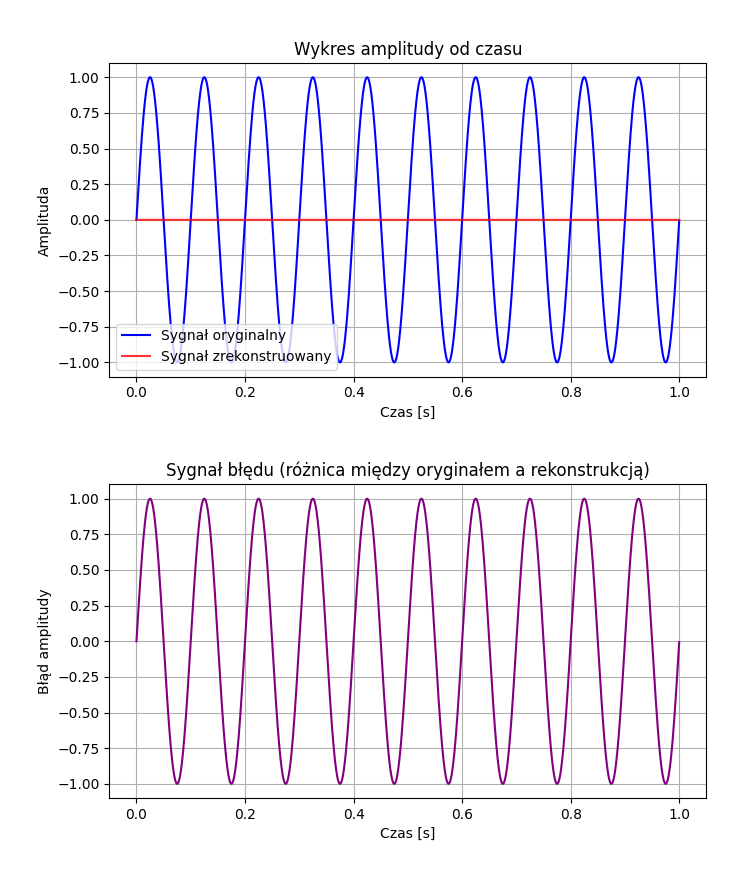
\includegraphics[width=0.85\linewidth]{exp1/new_f=10Hz.png}
    \caption{Wykres zrekonstruowanego przy nowej częstotliwości 10Hz}
    \label{fig:wykres_zrekonstruowanego_sygnalu_10Hz}
\end{figure}



% new_f = 40 Hz
% MSE: 0.3618
% SNR: 1.4050 dB
% PSNR: 4.4153 dB
% MD: 1.0078
% ENOB: -0.0590 bitów

\begin{table}[H]
    \centering
    \vspace{0.2cm}
    \begin{tabular}{|l|c|}
        \hline
        \textbf{Parametr} & \textbf{Wartość} \\ \hline
        \multicolumn{2}{|c|}{\textit{Parametry wejściowe}} \\ \hline
        Częstotliwość próbkowania ($f$) [Hz] & 40.0 \\ \hline
        Liczba bitów kwantyzacji (b) & 8 \\ \hline

        \multicolumn{2}{|c|}{\textit{Miary błędów}} \\ \hline
        MSE & 0.3618 \\ \hline
        SNR ($dB$) & 1.4050 \\ \hline
        PSNR ($dB$) & 4.4153 \\ \hline
        MD & 1.0078 \\ \hline
        ENOB (b) & -0.0590 \\ \hline
    \end{tabular}
    \caption{Parametry i miary błędów po konwersji}
    \label{tab:wyniki_rekonstrukcji_40Hz}
\end{table}

\begin{figure}[H]
    \centering
    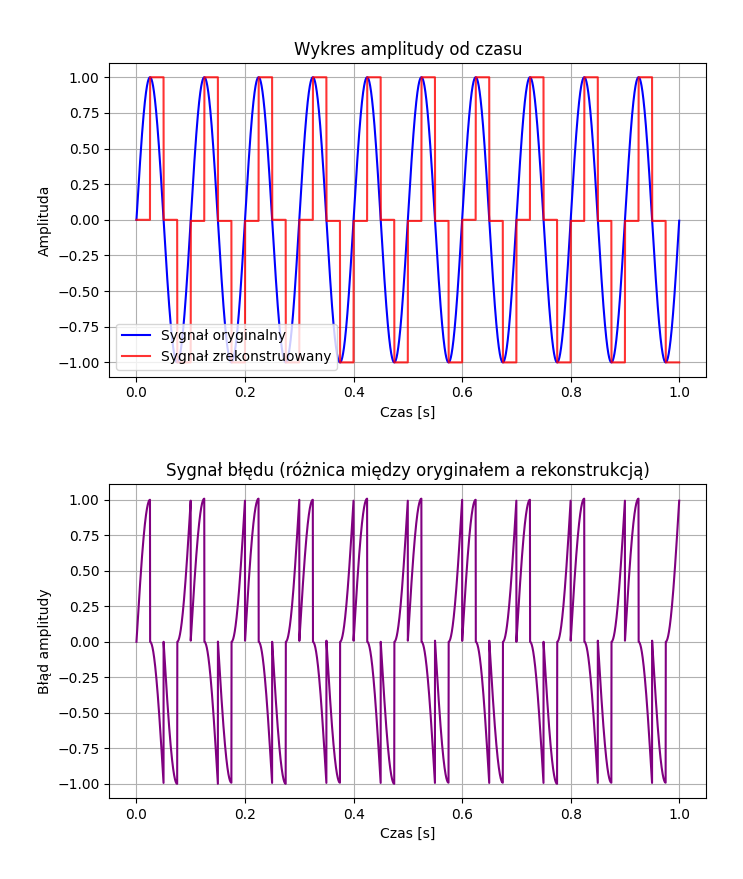
\includegraphics[width=0.85\linewidth]{exp1/new_f=40Hz.png}
    \caption{Wykres zrekonstruowanego przy nowej częstotliwości 40Hz}
    \label{fig:wykres_zrekonstruowanego_sygnalu_40Hz}
\end{figure}


% new_f = 400 Hz
% MSE: 0.0039
% SNR: 21.0739 dB
% PSNR: 24.0842 dB
% MD: 0.1580
% ENOB: 3.2083 bitów

\begin{table}[H]
    \centering
    \vspace{0.2cm}
    \begin{tabular}{|l|c|}
        \hline
        \textbf{Parametr} & \textbf{Wartość} \\ \hline
        \multicolumn{2}{|c|}{\textit{Parametry wejściowe}} \\ \hline
        Częstotliwość próbkowania ($f$) [Hz] & 400.0 \\ \hline
        Liczba bitów kwantyzacji (b) & 8 \\ \hline

        \multicolumn{2}{|c|}{\textit{Miary błędów}} \\ \hline
        MSE & 0.0039 \\ \hline
        SNR ($dB$) & 21.0739 \\ \hline
        PSNR ($dB$) & 24.0842 \\ \hline
        MD & 0.1580 \\ \hline
        ENOB (b) & 3.2083 \\ \hline
    \end{tabular}
    \caption{Parametry i miary błędów po konwersji}
    \label{tab:wyniki_rekonstrukcji_400Hz}
\end{table}

\begin{figure}[H]
    \centering
    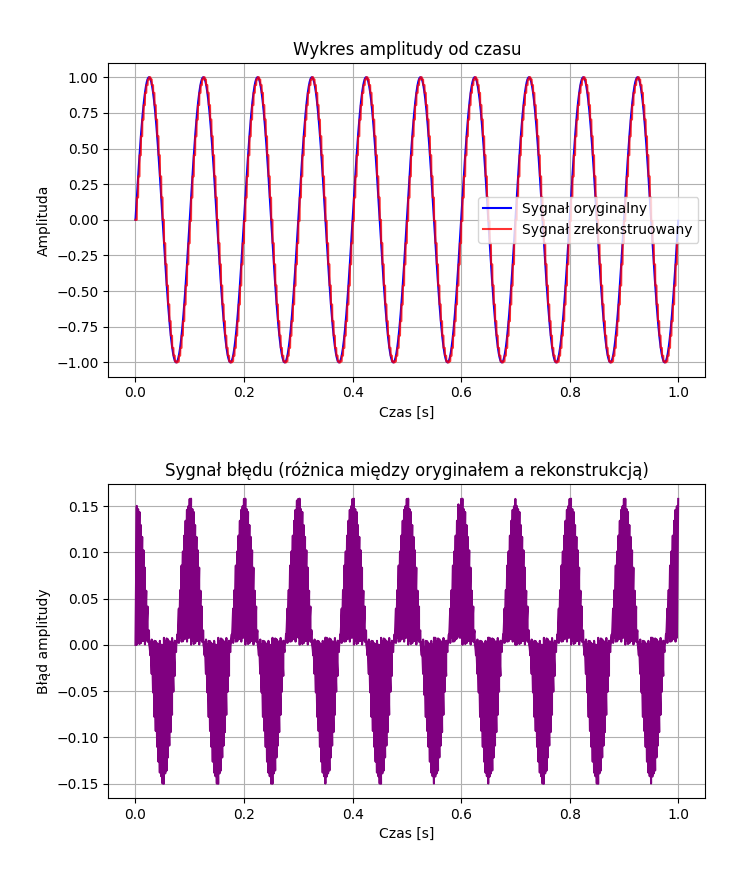
\includegraphics[width=0.85\linewidth]{exp1/new_f=400Hz.png}
    \caption{Wykres zrekonstruowanego przy nowej częstotliwości 400Hz}
    \label{fig:wykres_zrekonstruowanego_sygnalu_400Hz}
\end{figure}

Wnioski: 

\begin{itemize}
\item \textbf{Wpływ twierdzenia Nyquista-Shannona:} Sygnał oryginalny ma częstotliwość 10 Hz, co oznacza, że minimalna częstotliwość próbkowania pozwalająca na jego odtworzenie to 20 Hz.
Użycie częstotliwości 10 Hz (Tab. \ref{tab:wyniki_rekonstrukcji_10Hz}) łamie ten warunek, co prowadzi do  utraty informacji o sygnale, co pokazuje wykres (Rys. \ref{tab:wyniki_rekonstrukcji_10Hz}) oraz miary błędów: wysoki błąd średniokwadratowy ($MSE = 0.5$) oraz zerowy stosunek sygnału do szumu ($SNR = 0.0$ dB).

\item \textbf{Niedoskonałości ekstrapolacji zerowego rzędu (ZOH):} Metoda ZOH polega na utrzymywaniu stałej wartości próbki aż do momentu pobrania kolejnej, co tworzy widoczne schodki. Z tego powodu, przy małej częstotliwości (40 Hz) spełniającej warunek Nyquista, rekonstrukcja wciąż jest obarczona znacznym błędem ($MSE = 0.3618$, $SNR = 1.4050$ dB) (Tab. \ref{tab:wyniki_rekonstrukcji_40Hz}). Prosta funkcja schodkowa nie jest w stanie płynnie odwzorować dynamicznych zmian sygnału sinusoidalnego przy niewielkiej liczbie próbek na okres.

\item \textbf{Zalety nadpróbkowania:} Znaczne częstotliwości próbkowania do 400 Hz (Tab. \ref{tab:wyniki_rekonstrukcji_400Hz}) skutkuje dużą poprawą jakości odtworzonego sygnału. Błąd $MSE$ spada prawie do zera ($0.0039$), a parametr $SNR$ rośnie do ponad $21$ dB. Przy takim próbkowaniu stopnie generowane przez metodę ZOH stają się na bardzo małe, wykres zrekonstruowanego sygnału w wysokim stopniu aproksymuje oryginalny przebieg ciągły.

\item \textbf{Wniosek końcowy:} Jakość rekonstrukcji sygnału przy użyciu metody ekstrapolacji zerowego rzędu jest silnie uzależniona od częstotliwości próbkowania. Im wyższa jest ta częstotliwość, tym mniejszy wpływ ma niedoskonałość schodkowej natury ZOH, co przekłada się na niższe wartości błędów ($MSE$, $MD$) oraz wyższe wartości wskaźników jakościowych ($SNR$, $PSNR$).
\end{itemize}


\subsection{Eksperyment nr 2: Porównanie metod rekonstrukcji (ZOH i Sinc)}


Cel: porównanie zachowań przy dwóch różnych metodach rekonstrukcji w niskiej częstotliwości próbkowania. Dodatkowo zbadany zostanie wpływ szerokości okna w metodzie Sinc na dokładność rekonstrukcji.

W czasie trwania eksperymentu wykonano konwersję sygnału używając różnych metod i parametrów. Zostały one przedstawione wraz z wynikami miar błędów w poniższych tabelach.

% Metoda: ZOH, new_f = 40 Hz
% MSE: 0.3618
% SNR: 1.4052 dB
% PSNR: 4.4155 dB
% MD: 1.0000
% ENOB: -0.0589 bitów

\begin{table}[H]
    \centering
    \vspace{0.2cm}
    \begin{tabular}{|l|c|}
        \hline
        \textbf{Parametr} & \textbf{Wartość} \\ \hline
        \multicolumn{2}{|c|}{\textit{Parametry wejściowe}} \\ \hline
        Częstotliwość próbkowania ($f$) [Hz] & 40.0 \\ \hline
        Metoda rekonstrukcji & ZOH \\ \hline
        
        \multicolumn{2}{|c|}{\textit{Miary błędów}} \\ \hline
        MSE & 0.3618 \\ \hline
        SNR ($dB$) & 1.4052 \\ \hline
        PSNR ($dB$) & 4.4155 \\ \hline
        MD & 1.0000 \\ \hline
        ENOB (b) & -0.0589 \\ \hline
    \end{tabular}
    \caption{Parametry i miary błędów po konwersji (Metoda ZOH)}
    \label{tab:wyniki_zoh_40Hz}
\end{table}

\begin{figure}[H]
    \centering
    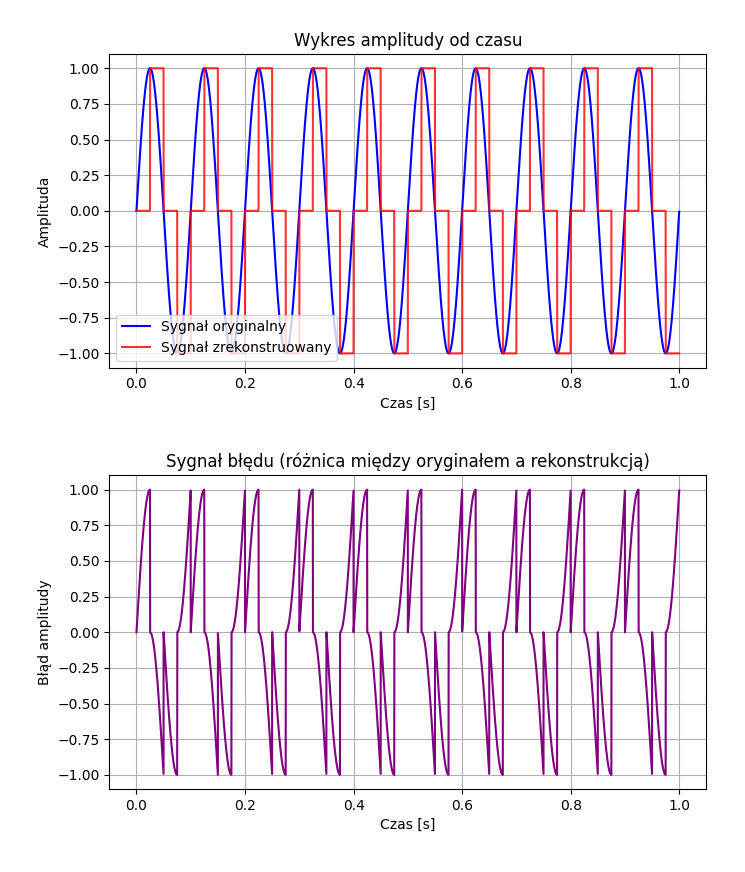
\includegraphics[width=0.85\linewidth]{exp2/zoh_40hz.png}
    \caption{Wykres zrekonstruowanego sygnału przy użyciu metody ZOH (40 Hz)}
    \label{fig:wykres_zoh_40hz}
\end{figure}

% Metoda: Sinc, okno = 20, new_f = 40 Hz
% MSE: 0.0011
% SNR: 26.4639 dB
% PSNR: 29.4742 dB
% MD: 0.1682
% ENOB: 4.1036 bitów

\begin{table}[H]
    \centering
    \vspace{0.2cm}
    \begin{tabular}{|l|c|}
        \hline
        \textbf{Parametr} & \textbf{Wartość} \\ \hline
        \multicolumn{2}{|c|}{\textit{Parametry wejściowe}} \\ \hline
        Częstotliwość próbkowania ($f$) [Hz] & 40.0 \\ \hline
        Metoda rekonstrukcji & Sinc (okno = 20) \\ \hline
        
        \multicolumn{2}{|c|}{\textit{Miary błędów}} \\ \hline
        MSE & 0.0011 \\ \hline
        SNR ($dB$) & 26.4639 \\ \hline
        PSNR ($dB$) & 29.4742 \\ \hline
        MD & 0.1682 \\ \hline
        ENOB (b) & 4.1036 \\ \hline
    \end{tabular}
    \caption{Parametry i miary błędów po konwersji (Sinc, okno=20)}
    \label{tab:wyniki_sinc_40Hz_w20}
\end{table}

\begin{figure}[H]
    \centering
    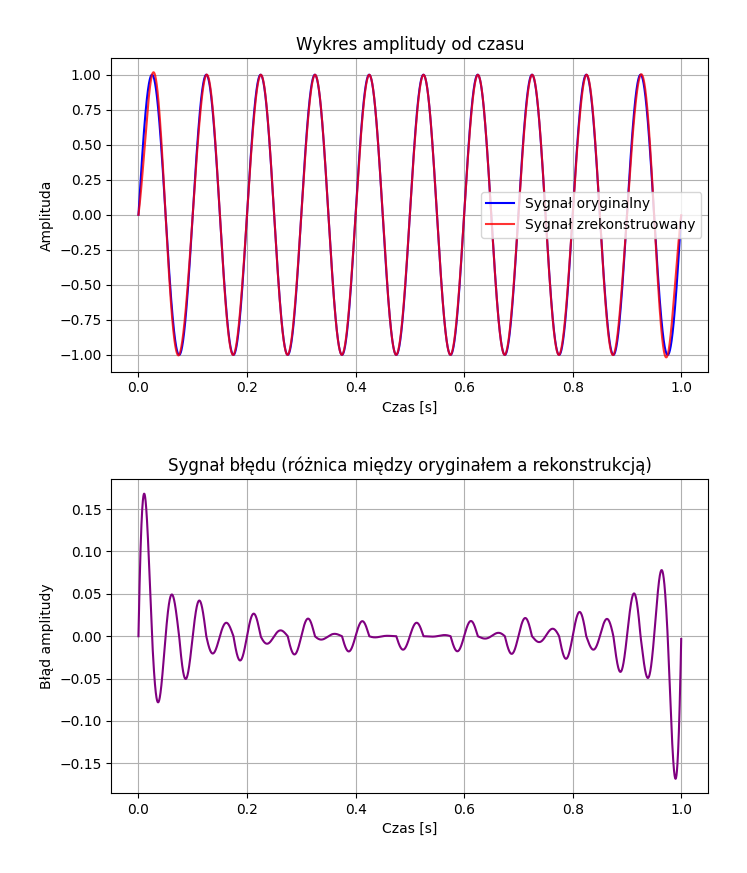
\includegraphics[width=0.85\linewidth]{exp2/sinc_40hz_w20.png}
    \caption{Wykres zrekonstruowanego sygnału przy użyciu funkcji Sinc (okno=20)}
    \label{fig:wykres_sinc_40hz_w20}
\end{figure}

% Metoda: Sinc, okno = 200, new_f = 40 Hz
% MSE: 0.0012
% SNR: 26.1052 dB
% PSNR: 29.1155 dB
% MD: 0.1643
% ENOB: 4.0440 bitów

\begin{table}[H]
    \centering
    \vspace{0.2cm}
    \begin{tabular}{|l|c|}
        \hline
        \textbf{Parametr} & \textbf{Wartość} \\ \hline
        \multicolumn{2}{|c|}{\textit{Parametry wejściowe}} \\ \hline
        Częstotliwość próbkowania ($f$) [Hz] & 40.0 \\ \hline
        Metoda rekonstrukcji & Sinc (okno = 200) \\ \hline
        
        \multicolumn{2}{|c|}{\textit{Miary błędów}} \\ \hline
        MSE & 0.0012 \\ \hline
        SNR ($dB$) & 26.1052 \\ \hline
        PSNR ($dB$) & 29.1155 \\ \hline
        MD & 0.1643 \\ \hline
        ENOB (b) & 4.0440 \\ \hline
    \end{tabular}
    \caption{Parametry i miary błędów po konwersji (Sinc, okno=200)}
    \label{tab:wyniki_sinc_40Hz_w200}
\end{table}

\begin{figure}[H]
    \centering
    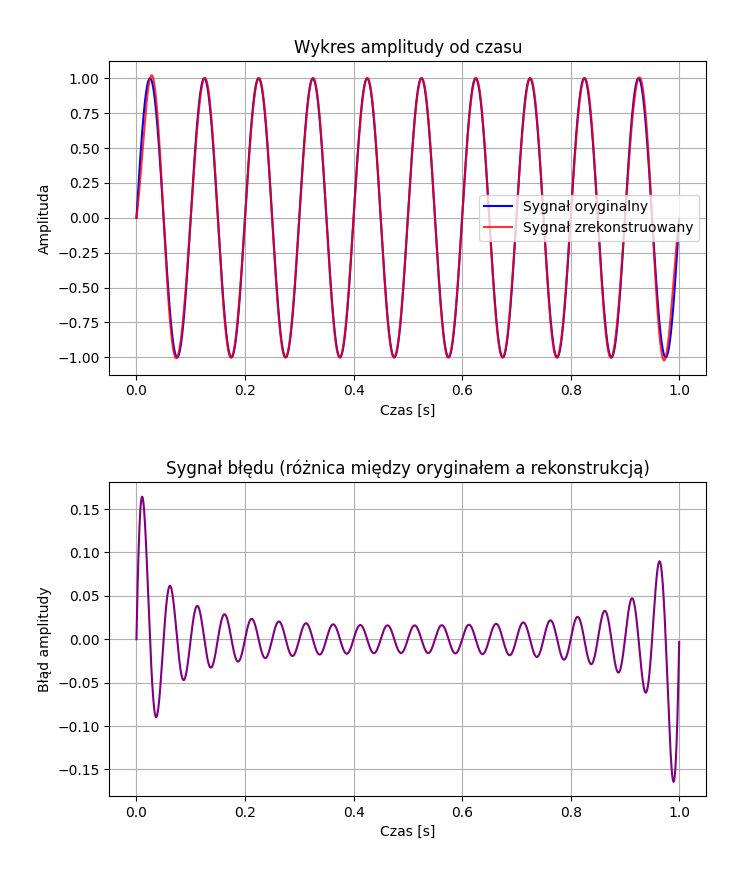
\includegraphics[width=0.85\linewidth]{exp2/sinc_40hz_w200.png}
    \caption{Wykres zrekonstruowanego sygnału przy użyciu funkcji Sinc (okno=200)}
    \label{fig:wykres_sinc_40hz_w200}
\end{figure}

Wnioski:
\begin{itemize}
    \item \textbf{Znaczna przewaga funkcji Sinc:} Przy tej samej, stosunkowo niskiej częstotliwości próbkowania (40 Hz), rekonstrukcja oparta na funkcji Sinc daje lepsze rezultaty niż ekstrapolacja zerowego rzędu. Błąd średniokwadratowy ($MSE$) dla metody ZOH wynosi aż $0.3618$, podczas gdy zastosowanie funkcji Sinc drastycznie redukuje go do poziomu $0.0011$. Z kolei wskaźnik stosunku sygnału do szumu ($SNR$) wzrasta z marginalnego $1.4$ dB dla ZOH do blisko $26.5$ dB dla metody Sinc.
    \item \textbf{Wpływ szerokości okna w metodzie Sinc:} Zwiększenie szerokości okna z 20 do 200 próbek nie przyniosło istotnej poprawy parametrów jakościowych. Co więcej, zauważalny jest minimalny spadek wartości $SNR$ z $26.46$ dB do $26.10$ dB oraz wzrost błędu $MSE$ z $0.0011$ do $0.0012$. Zjawisko to sugeruje, że dla analizowanego sygnału okno o szerokości 20 jest optymalne, a zbyt szerokie okno uwzględnia odległe czasowo próbki, co w połączeniu z efektem obcięcia sygnału na brzegach analizowanego przedziału może wprowadzać nieznaczne błędy.
    \item \textbf{Podsumowanie ogólne:} Zjawisko gwałtownego „schodkowania” w ZOH w znacznym stopniu degraduje sygnał. Aby metoda ZOH mogła konkurować jakościowo z metodą Sinc przy odtwarzaniu ciągłych przebiegów, wymagałaby zastosowania ogromnego nadpróbkowania, co zwiększyłoby koszty obliczeniowe.
\end{itemize}

\subsection{Eksperyment nr 3: Zjawisko aliasingu w pasmach częstotliwościowych}
Cel: udowodnienie, że niedostateczna częstotliwość próbkowania sprawia, iż nie da się odróżnić sygnału $f_0$ od sygnału $f_d$, gdzie $f_d = f_0 + k f_s$. Zbadano sygnał, którego częstotliwość próbkowania $f_s = 1000$ Hz, częstotliwość sygnału bazowego $f_0 = 100$ Hz oraz wyznaczona częstotliwość aliasująca $f_d = f_0 + 1 \cdot f_s = 1100$ Hz.

Eksperyment podzielono na dwa etapy. W obu przypadkach do konwersji użyto tej samej częstotliwości próbkowania ($f_s = 1000$ Hz) oraz metody rekonstrukcji opartej na funkcji Sinc. Użyto 16-bitowej kwantyzacji, aby wyeliminować wpływ błędu (szumu) kwantyzacji na badane zjawisko.

\subsubsection*{Etap 1: Próbkowanie sygnału bazowego ($f_0 = 100$ Hz)}

W pierwszym kroku wygenerowano i poddano konwersji sygnał o częstotliwości 100 Hz. Ponieważ $1000 \text{ Hz} > 2 \cdot 100 \text{ Hz}$, warunek Nyquista jest tutaj spełniony.

\begin{table}[H]
    \centering
    \vspace{0.2cm}
    \begin{tabular}{|l|c|l|c|}
        \hline
        \multicolumn{2}{|c|}{\textbf{Parametry generatora sygnału}} & \multicolumn{2}{|c|}{\textbf{Parametry konwersji (A/C i C/A)}} \\ \hline
        Amplituda ($A$) & 1.0 & Częstotliwość próbkowania $f_s$ [Hz] & 1000.0 \\ \hline
        Czas początkowy ($t_1$) [s] & 0.0 & Liczba bitów kwantyzacji (b) & 16 \\ \hline
        Czas trwania ($d$) [s] & 0.05 & Metoda rekonstrukcji & Sinc (okno = 20) \\ \hline
        Częstotliwość ($f_{gen}$) [kHz] & 10.0 & & \\ \hline
        Częstotliwość sygnału $f_0$ [Hz] & \textbf{100.0} & & \\ \hline
        Przesunięcie fazowe [rad] & 0.0 & & \\ \hline
    \end{tabular}
    \caption{Parametry dla Etapu 1 (Sygnał bazowy 100 Hz)}
    \label{tab:parametry_aliasing_100Hz}
\end{table}

 \begin{figure}[H]
     \centering
     % UWAGA: Wygeneruj wykresy w programie i podmień nazwy plików
     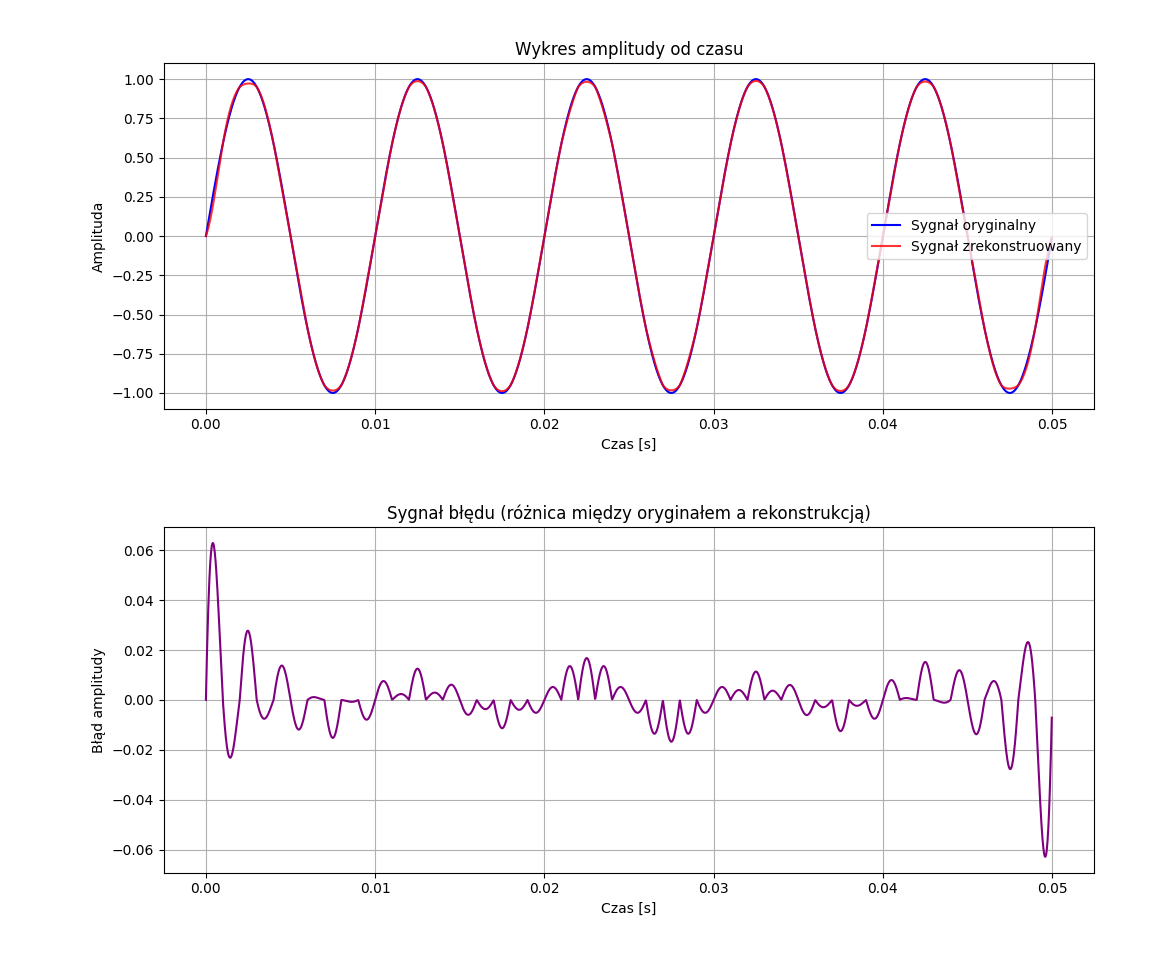
\includegraphics[width=0.85\linewidth]{exp3/sygnal_100hz_org.png}
     \caption{Oryginalny sygnał ciągły 100 Hz, oraz zrekonstruowany sygnał (próbkowanie 1000 Hz).}
     \label{fig:wykresy_aliasing_100Hz}
 \end{figure}

\textit{Zanotowane miary błędów dla Etapu 1: MSE: ~0.0000, SNR: bardzo wysokie (powyżej 50 dB). Sygnał został odtworzony poprawnie.}

\vspace{0.5cm}

\subsubsection*{Etap 2: Próbkowanie sygnału aliasującego ($f_d = 1100$ Hz)}

W drugim kroku wygenerowano sygnał o częstotliwości 1100 Hz. Zgodnie z twierdzeniem Nyquista, minimalna częstotliwość próbkowania wynosiłaby 2200 Hz. Użyto jednak (celowo) tej samej częstotliwości konwersji $f_s = 1000$ Hz, co w Etapie 1.

\begin{table}[H]
    \centering
    \vspace{0.2cm}
    \begin{tabular}{|l|c|l|c|}
        \hline
        \multicolumn{2}{|c|}{\textbf{Parametry generatora sygnału}} & \multicolumn{2}{|c|}{\textbf{Parametry konwersji (A/C i C/A)}} \\ \hline
        Amplituda ($A$) & 1.0 & Częstotliwość próbkowania $f_s$ [Hz] & 1000.0 \\ \hline
        Czas początkowy ($t_1$) [s] & 0.0 & Liczba bitów kwantyzacji (b) & 16 \\ \hline
        Czas trwania ($d$) [s] & 0.05 & Metoda rekonstrukcji & Sinc (okno = 20) \\ \hline
        Częstotliwość ($f_{gen}$) [kHz] & 10.0 & & \\ \hline
        Częstotliwość sygnału $f_d$ [Hz] & \textbf{1100.0} & & \\ \hline
        Przesunięcie fazowe [rad] & 0.0 & & \\ \hline
    \end{tabular}
    \caption{Parametry dla Etapu 2 (Sygnał aliasujący 1100 Hz)}
    \label{tab:parametry_aliasing_1100Hz}
\end{table}

 \begin{figure}[H]
     \centering
     % UWAGA: Wygeneruj wykresy w programie i podmień nazwy plików
     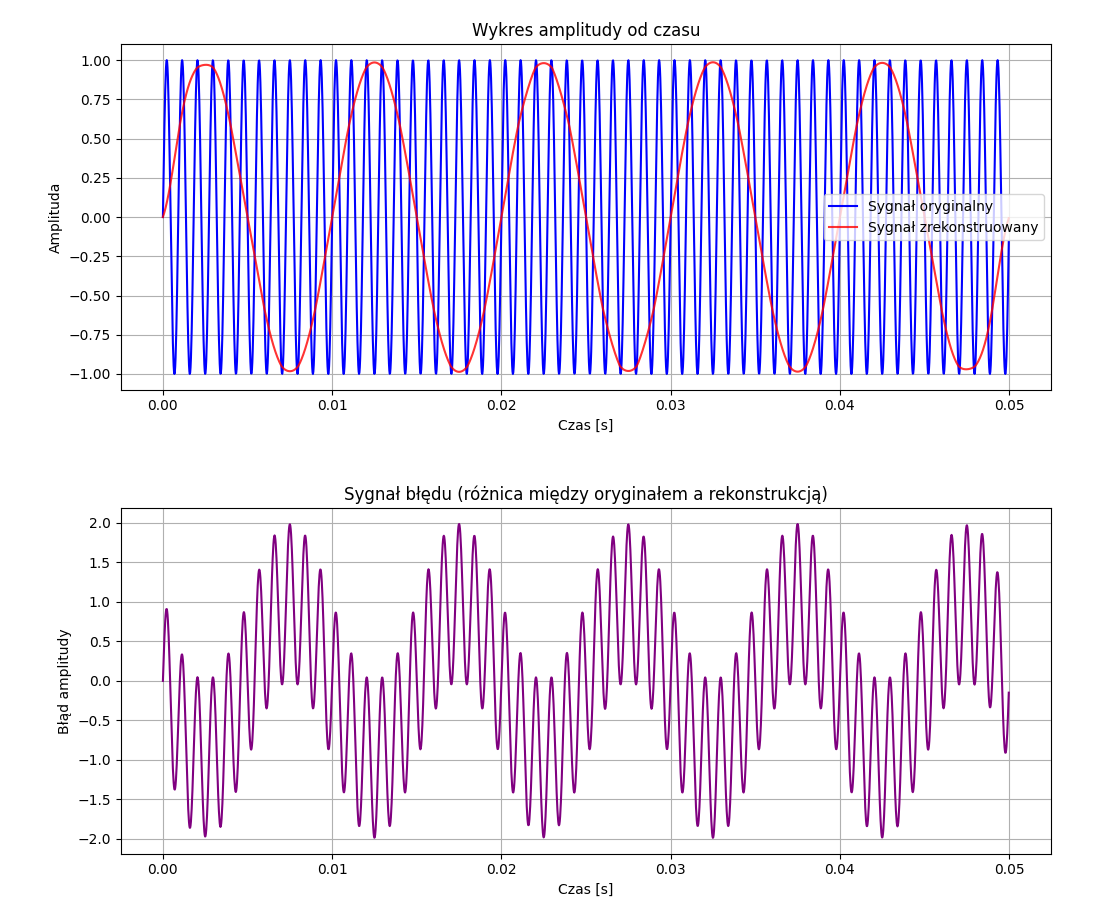
\includegraphics[width=0.85\linewidth]{exp3/sygnal_1100hz_org.png}
     \caption{Oryginalny sygnał ciągły 1100 Hz, oraz zrekonstruowany sygnał (próbkowanie 1000 Hz).}
     \label{fig:wykresy_aliasing_1100Hz}
 \end{figure}

\textit{Zanotowane miary błędów dla Etapu 2: Błąd MSE dla tego etapu przyjął wartość bardzo wysoką (np. > 0.5), a parametr SNR spadł poniżej zera (wskazując całkowitą degradację).}

\vspace{0.5cm}

\subsubsection*{Wnioski}
\begin{itemize}
    \item \textbf{Dowód na istnienie aliasingu:} Jak można zauważyć na rysunku \ref{fig:wykresy_aliasing_1100Hz} (po prawej stronie), przetwornik A/C spróbkował gęsty sygnał 1100 Hz w taki sposób, że zrekonstruowany z niego przebieg wygląda \textbf{identycznie} jak sygnał o częstotliwości 100 Hz z pierwszego etapu eksperymentu (Rys. \ref{fig:wykresy_aliasing_100Hz}). 
    \item \textbf{Przyczyna zjawiska:} Zjawisko to wynika z matematycznych właściwości próbkowania. Próbki pobierane co $1/1000$ sekundy trafiają w te same wartości amplitudy dla funkcji trygonometrycznej $\sin(2\pi \cdot 100 \cdot t)$ oraz $\sin(2\pi \cdot 1100 \cdot t)$.
    \item \textbf{Interpretacja miar błędów:} W Etapie 2 błąd MSE jest ogromny, ponieważ program porównuje odtworzony (na skutek aliasingu) sygnał 100 Hz z wygenerowanym w tle, gęstym sygnałem wzorcowym 1100 Hz. Różnica między nimi jest drastyczna.
    \item \textbf{Aspekt praktyczny:} Eksperyment potwierdza bezwzględną konieczność stosowania analogowych filtrów dolnoprzepustowych (antyaliasingowych) przed przetwornikiem A/C w urządzeniach rzeczywistych. Gdyby do systemu wpadł zakłócający sygnał o częstotliwości 1100 Hz, po spróbkowaniu komputer błędnie zinterpretowałby go jako sygnał użyteczny 100 Hz, bez możliwości odróżnienia od fałszu.
\end{itemize}


\section{Wnioski}

\subsection*{Wnioski szczegółowe z eksperymentów}

\subsubsection*{1. Znaczenie częstotliwości próbkowania}
Eksperymenty 1 i 2 dowiodły, że częstotliwość próbkowania jest kluczowym parametrem determinującym jakość rekonstrukcji sygnału. Przy próbkowaniu poniżej granicy Nyquista ($f_s < 2 f_{max}$) metoda ZOH wprowadza znaczne zniekształcenia (MSE = 0.3618 dla 40 Hz). Zastosowanie rekonstrukcji opartej na funkcji Sinc drastycznie poprawia wyniki nawet przy niskiej częstotliwości próbkowania (MSE = 0.0011 dla tej samej konfiguracji). Zarówno metoda ZOH, jak i Sinc wymagają jednak wystarczająco wysokiej próbkowania — algorytm ZOH potrzebuje znacznego nadpróbkowania, a metoda Sinc pozostaje efektywna przy rozsądnym dobieraniu okien (szerokość okna 20 vs 200 nie daje istotnej poprawy).

\subsubsection*{2. Znaczenie aliasingu}
Eksperyment 3 zademonstrował fundamentalne ograniczenie cyfrowego przetwarzania sygnałów — zjawisko aliasingu. Przy próbkowaniu sygnału 1100 Hz częstotliwością 1000 Hz, zrekonstruowany przebieg jest \textbf{praktycznie identyczny} z sygnałem 100 Hz próbkowanym tą samą częstotliwością. Matematycznie, próbki pobierane co $T_s = 1$ ms trafiają w te same amplitudy dla obu sygnałów, co wynika z periodyczności funkcji sinus. Błąd porównania (MSE >> 0.5, SNR << 0 dB) jest ogromny, ponieważ program porównuje odtworzony (aliasowany) sygnał 100 Hz z oryginalnym sygnałem 1100 Hz. W praktyce urządzenia cyfrowe nie mogą odróżnić oryginału od aliasu - wymagane są zatem filtry antyaliasingowe przed przetwornikiem A/C.

\subsubsection*{3. Znaczenie praktyczne}
Wszystkie eksperymenty potwierdzają, że projektowanie systemów akwizycji danych wymaga:
\begin{enumerate}
    \item Określenia maksymalnej częstotliwości sygnału ($f_{max}$) w aplikacji,
    \item Wyboru częstotliwości próbkowania $f_s > 2 f_{max}$ (reguła Nyquista),
    \item Stosowania filtrów dolnoprzepustowych przed A/C w celu eliminacji składowych powyżej $f_{max}$,
    \item Wybrania odpowiedniej metody rekonstrukcji sygnału w zależności od dostępnych zasobów obliczeniowych (ZOH dla szybkich operacji, Sinc dla wyższej jakości).
\end{enumerate}
Zaniedbanie któregokolwiek z tych warunków prowadzi do utraty informacji i uniemożliwia  wiarygodne odtworzenie oryginalnego przebiegu.


\begin{thebibliography}{1}
\bibitem{1} Instrukcja do zadania 2
\end{thebibliography}

\end{document}